% =====================================================================
% BLOQUES PARA PEGAR EN main.tex (Overleaf)
% Preparados el 20-oct-2026 con los datos de la campaña (18 y 20 de octubre).
% - Las figuras van en la carpeta "figuras" de Overleaf:
%     figuras/campana_llenados.png   y   figuras/campana_grupos.png
% - Los encabezados (\subsection, \subsubsection) se pueden cambiar de nivel
%   para que encajen con la estructura de su documento.
% - Lo marcado con PENDIENTE lo completan ustedes.
% - Paquetes que usa: graphicx (ya lo usan para las figuras). Nada más.
% =====================================================================


% ---------------------------------------------------------------------
% BLOQUE 1 — METODOLOGÍA (dentro de la Fase 4: integración y pruebas)
% ---------------------------------------------------------------------

\subsection{Protocolo de medición y diseño experimental}

\subsubsection{Muestras}

Como muestra de control se utilizó agua estéril para inyección, que no contiene
partículas en suspensión. Las muestras contaminadas se prepararon con la misma
agua y dos partículas de polietileno de color azul oscuro, de
PENDIENTE~mm y PENDIENTE~mm, que se ubicaron en la zona de medición del microcanal,
frente al fotodetector. Antes de cada llenado, las partículas se dejaron en remojo
para desprender el aire adherido a su superficie, y después de cada medición se
contaron al vaciar el chip para verificar que no quedaran atrapadas.

\subsubsection{Medición de un llenado}

Cada llenado del microcanal se midió con una secuencia automática del
microcontrolador. Primero, el LED trabaja durante 180~s sin que se guarden datos,
para que alcance su temperatura de operación. Después se realizan 10 repeticiones;
en cada una se toman 1000 muestras con el LED apagado y 1000 con el LED encendido, a
1000~muestras por segundo. La señal útil de cada repetición es la diferencia
\begin{equation}
  \Delta V = \mu_{\mathrm{encendido}} - \mu_{\mathrm{apagado}},
\end{equation}
que elimina el aporte de la luz ambiente y del nivel de reposo del fotodetector.
El resultado del llenado es el promedio de las 10 repeticiones. Cada medición
completa toma unos 3~min 20~s.

\subsubsection{Referencia de cada sesión}

Al inicio de cada sesión se midió el chip lleno con agua limpia durante 20~s
($\Delta V_{\mathrm{ref}}$), y al final se repitió la medición para comprobar que el
instrumento no hubiera cambiado. Para poder comparar sesiones y chips distintos, cada
llenado se expresa como porcentaje de la referencia de su sesión:
\begin{equation}
  T_{\mathrm{rel}} = \frac{\Delta V}{\Delta V_{\mathrm{ref}}} \times 100\,\%.
\end{equation}

\subsubsection{Control de burbujas y orden de las muestras}

En una prueba piloto aparecieron caídas de señal en llenados de agua limpia, del
mismo tamaño que las producidas por las partículas, asociadas a burbujas en la zona
de medición. Por eso se estableció un procedimiento de llenado: la jeringa se purga antes de usarla, el chip se llena
inclinado desde el extremo más bajo para que el aire salga por el extremo alto, y la
zona de medición se revisa a contraluz antes de cada medición. Si hay una burbuja,
el chip se vacía y se vuelve a llenar. Las muestras se midieron en orden alternado
(agua limpia, agua con PE, agua limpia, \dots) para que una deriva lenta del
instrumento no favoreciera a ninguno de los dos grupos.

\subsubsection{Regla de descarte}

Antes de iniciar la campaña se definió que un llenado solo puede descartarse por una
falla física anotada en el momento (por ejemplo, una filtración del chip o un chip
mal insertado), o porque el firmware lo marque como saturado. Ningún llenado se
descartó por el valor obtenido. Los llenados descartados se conservan en los
registros con el motivo.

\subsubsection{Criterio de detección y análisis estadístico}

También antes de la campaña se fijó el criterio de clasificación: un llenado se
considera \emph{con presencia probable de partículas} si
$\Delta V < 0{,}8\,\Delta V_{\mathrm{ref}}$, es decir, si la transmisión relativa cae
por debajo del 80\,\%. El umbral deja un margen amplio frente a la variación normal
entre llenados de agua limpia, que es de alrededor del 3--4\,\%.

Para el análisis estadístico se tomó un único valor por llenado ($T_{\mathrm{rel}}$),
ya que las 10 repeticiones de un mismo llenado no son independientes entre sí. Los
dos grupos se compararon con la prueba $t$ de Welch, una variante de la prueba
$t$ de Student que no supone varianzas iguales, con un nivel de significancia de
0,05. Como comprobación, se aplicó también la prueba no paramétrica de Mann-Whitney.
El desempeño del criterio de detección se resumió en una matriz de confusión, con la
sensibilidad y la especificidad acompañadas de su intervalo de confianza del 95\,\%
(método exacto de Clopper-Pearson). La condición real de cada llenado se verificó con
las fotografías a contraluz tomadas antes y después de cada medición. El
procesamiento se hizo con un programa en Python (bibliotecas SciPy y Matplotlib, de
uso libre).


% ---------------------------------------------------------------------
% BLOQUE 2 — RESULTADOS: AGUA LIMPIA FRENTE A AGUA CON PE
% ---------------------------------------------------------------------

\subsection{Validación: agua limpia frente a agua con polietileno}

La campaña se realizó en tres sesiones, con dos chips: dos sesiones el 18 de
octubre con el chip~1 y una sesión el 20 de octubre con el chip~2. En total se
obtuvieron 22 llenados válidos: 11 con agua limpia y 11 con partículas de PE. Las
referencias de las sesiones fueron 2221, 2179 y 2002~cuentas. La diferencia entre
ellas, de hasta un 10\,\%, se debe principalmente al cambio de chip, y queda
compensada al expresar cada llenado como porcentaje de su propia referencia. En la sesión del chip~2, la
medición de cierre quedó a 0,23\,\% de la inicial, lo que confirma que el
instrumento se mantuvo estable durante la sesión.

Dentro de cada llenado, la señal fue muy estable: la incertidumbre del promedio de
$\Delta V$ estuvo entre 0,09 y 0,50~cuentas, y la variación entre las 10 repeticiones
no superó el 0,34\,\% del valor medido. La Figura~\ref{fig:campana_llenados} muestra
todos los llenados en el orden en que se midieron.

\begin{figure}[htbp]
  \centering
  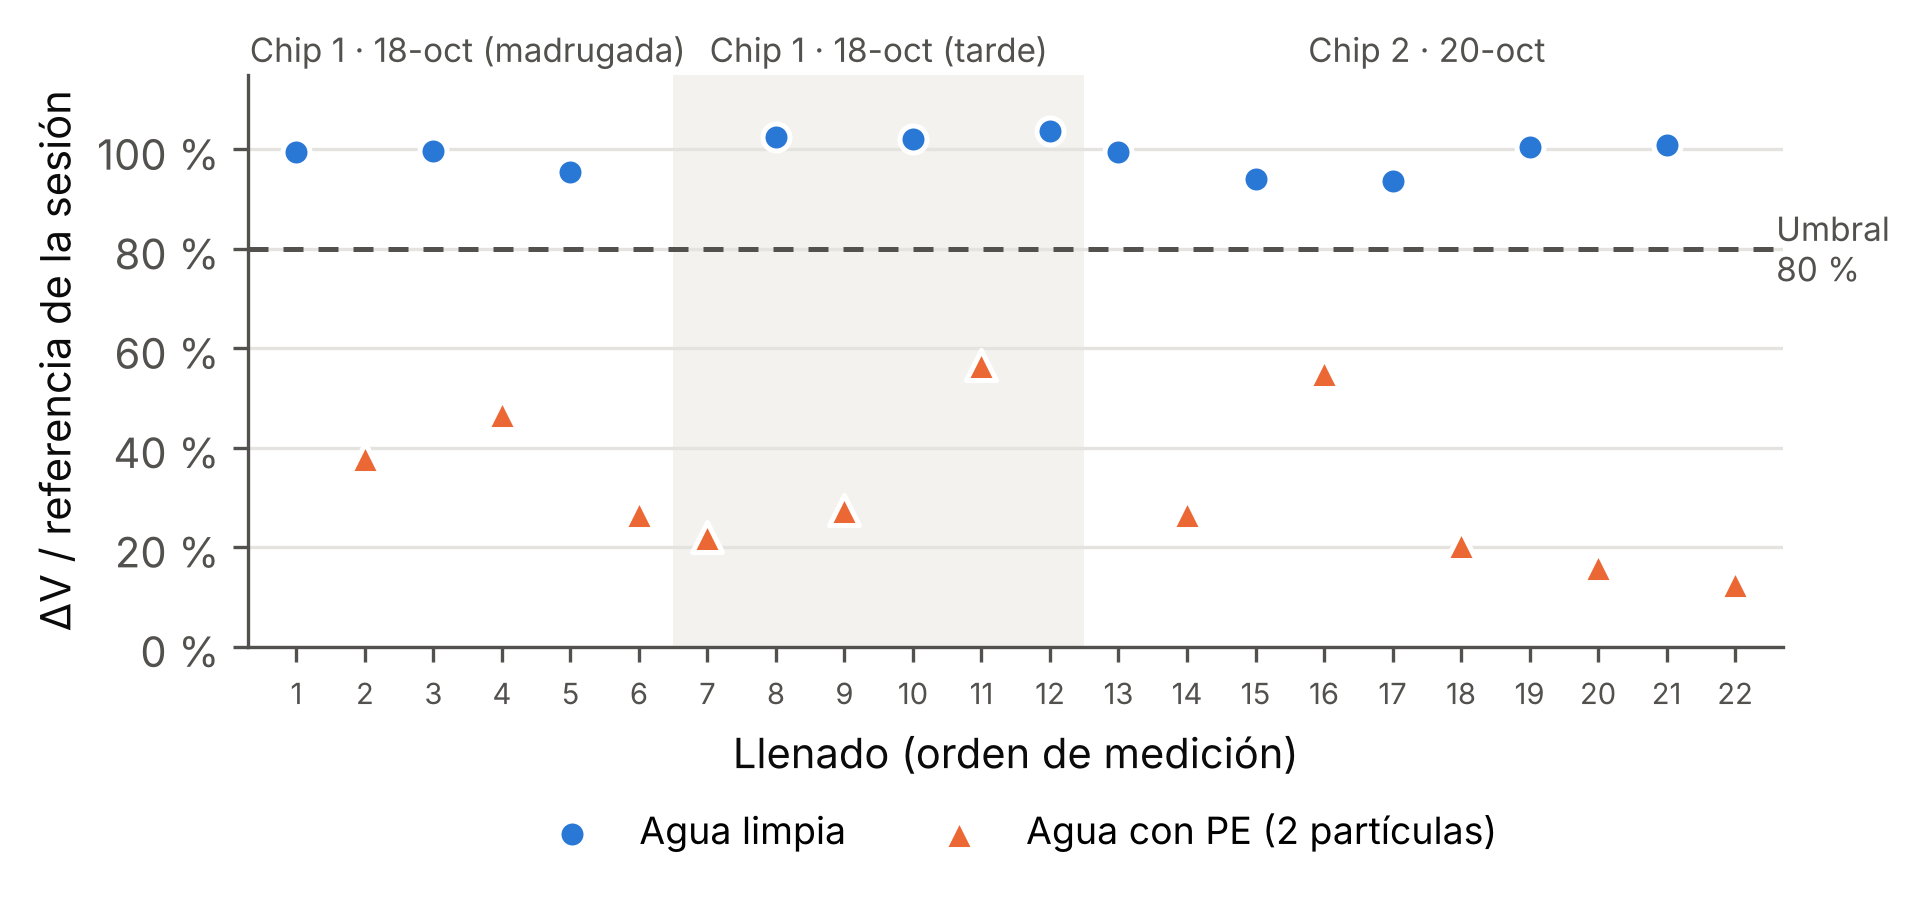
\includegraphics[width=\textwidth]{figuras/campana_llenados.png}
  \caption{Transmisión relativa de cada llenado válido, en orden de medición. Los
    círculos corresponden a agua limpia y los triángulos a agua con dos partículas
    de PE. La línea discontinua marca el umbral de detección (80\,\%).}
  \label{fig:campana_llenados}
\end{figure}

Todos los llenados de agua limpia quedaron entre 93,7\,\% y 103,7\,\% de la
referencia, y todos los llenados con PE quedaron entre 12,6\,\% y 56,7\,\%. Los dos
grupos no se superponen: el llenado limpio más bajo quedó 13,7 puntos por encima del
umbral, y el llenado con PE más alto, 23,3 puntos por debajo. La
Tabla~\ref{tab:campana_resumen} resume los resultados por chip y en total, y la
Figura~\ref{fig:campana_grupos} los compara por grupo.

\begin{table}[htbp]
  \centering
  \caption{Transmisión relativa por grupo y por chip (un valor por llenado).}
  \label{tab:campana_resumen}
  \begin{tabular}{lcccc}
    \hline
    Grupo & Chip & $n$ & Media (\%) & Desv. estándar (\%) \\
    \hline
    Agua limpia & 1 & 6  & 100,5 & 3,0  \\
    Agua limpia & 2 & 5  & 97,8  & 3,6  \\
    Agua limpia & Total & 11 & 99,3 & 3,4 \\
    \hline
    Agua con PE & 1 & 6  & 36,3  & 13,4 \\
    Agua con PE & 2 & 5  & 26,2  & 16,9 \\
    Agua con PE & Total & 11 & 31,7 & 15,2 \\
    \hline
  \end{tabular}
\end{table}

\begin{figure}[htbp]
  \centering
  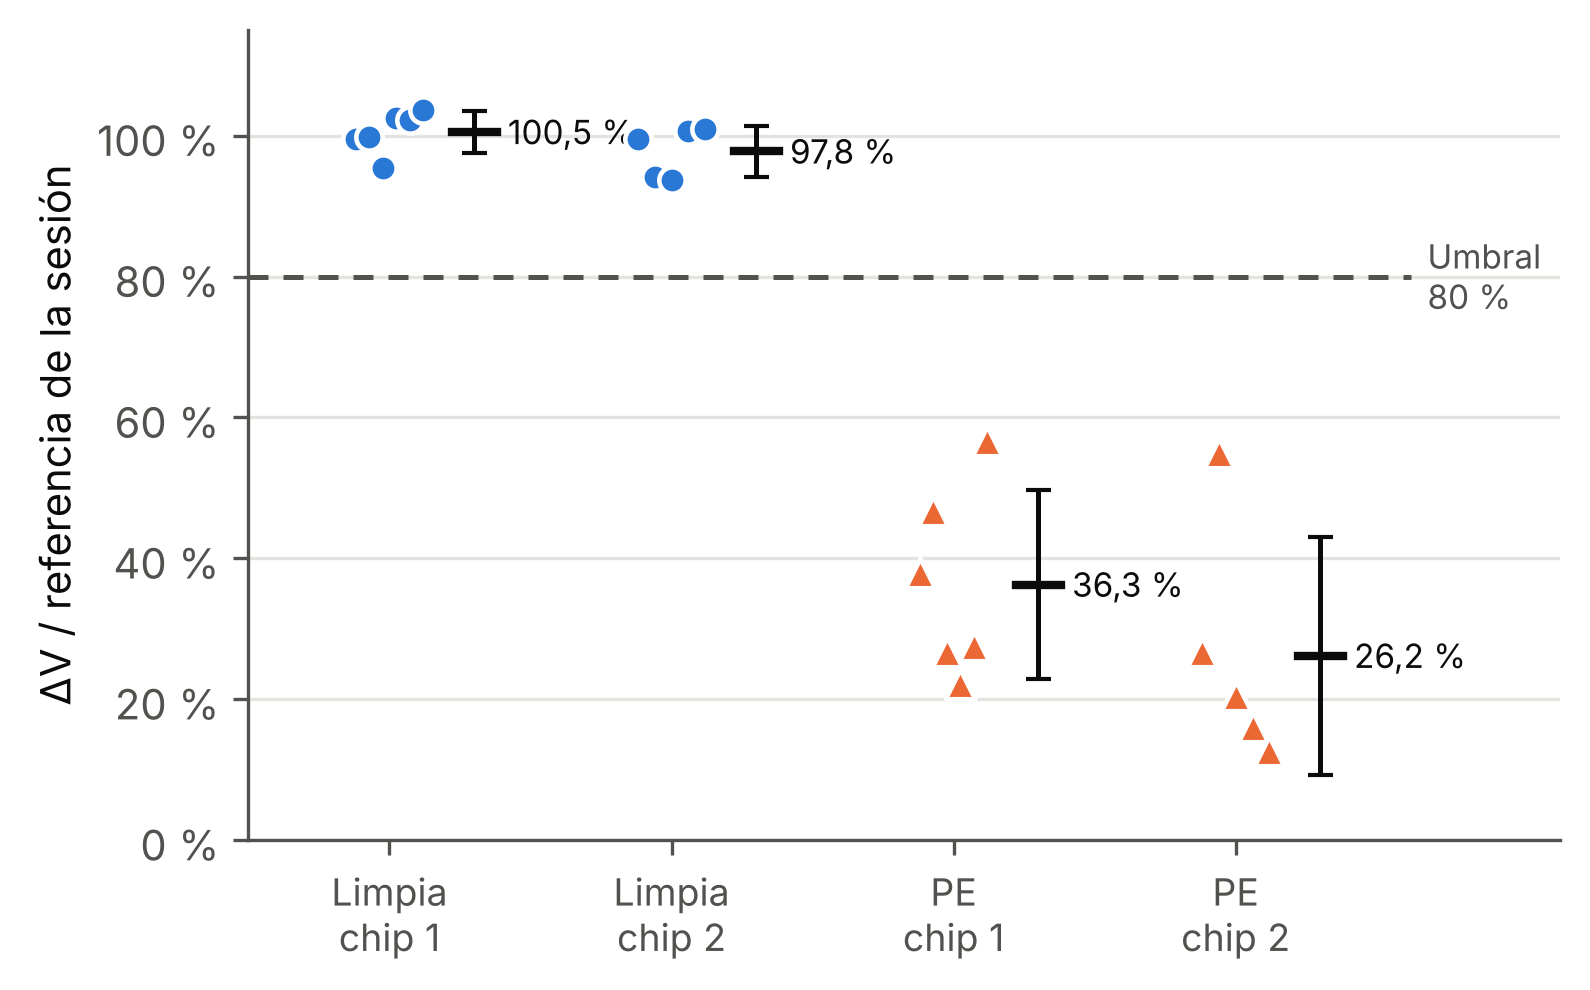
\includegraphics[width=0.8\textwidth]{figuras/campana_grupos.png}
  \caption{Transmisión relativa por grupo y por chip. Cada punto es un llenado; la
    barra horizontal indica la media y las barras verticales, una desviación estándar.}
  \label{fig:campana_grupos}
\end{figure}

En promedio, la presencia de las partículas de PE redujo la señal en un 68\,\%. La
prueba $t$ de Welch muestra que la diferencia entre los grupos es estadísticamente
significativa en cada chip por separado y en el conjunto
(Tabla~\ref{tab:campana_welch}). La prueba de Mann-Whitney confirma el resultado
($p = 8{,}2 \times 10^{-5}$).

\begin{table}[htbp]
  \centering
  \caption{Prueba $t$ de Welch entre agua limpia y agua con PE (transmisión relativa).}
  \label{tab:campana_welch}
  \begin{tabular}{lccccc}
    \hline
    Conjunto & $t$ & g.\,l. & $p$ & Diferencia & IC 95\,\% \\
     &  &  &  & (puntos) & (puntos) \\
    \hline
    Chip 1 & 11,5 & 5,5  & $4{,}9 \times 10^{-5}$ & 64,2 & 50,2 a 78,3 \\
    Chip 2 & 9,3  & 4,4  & $5{,}0 \times 10^{-4}$ & 71,6 & 50,8 a 92,4 \\
    Total  & 14,4 & 11,0 & $1{,}8 \times 10^{-8}$ & 67,6 & 57,2 a 78,0 \\
    \hline
  \end{tabular}
\end{table}

Con el umbral del 80\,\%, los 22 llenados quedaron bien clasificados
(Tabla~\ref{tab:campana_confusion}): 11 verdaderos positivos y 11 verdaderos
negativos, sin falsos positivos ni falsos negativos. La sensibilidad y la
especificidad observadas fueron del 100\,\%. Con 11 casos por grupo, el intervalo de
confianza del 95\,\% de cada una va del 71,5\,\% al 100\,\%, y el de la exactitud
(22 de 22), del 84,6\,\% al 100\,\%. Para estimar estos indicadores con mayor
precisión se requerirían más llenados.

\begin{table}[htbp]
  \centering
  \caption{Matriz de confusión del criterio de detección (umbral del 80\,\%).}
  \label{tab:campana_confusion}
  \begin{tabular}{lcc}
    \hline
     & \multicolumn{2}{c}{Clasificación del prototipo} \\
    Condición real & Presencia probable de PE & Sin partículas \\
    \hline
    Con PE (11)      & 11 & 0  \\
    Agua limpia (11) & 0  & 11 \\
    \hline
  \end{tabular}
\end{table}

La señal de los llenados con PE varió más que la del agua limpia (desviación
estándar de 15,2 puntos frente a 3,4). Esto se explica porque la atenuación depende
de la posición y la orientación con que quedan las partículas frente al haz, que no
son iguales en cada llenado (véanse las fotografías a contraluz). Aun así, ningún
llenado con PE se acercó al umbral.

Durante la campaña se descartaron tres llenados por fallas físicas anotadas en el
momento: uno por una filtración del chip~1 durante la medición, que obligó a cambiar
de chip, y dos realizados con un chip que presentaba fugas. Además, varias
mediciones se cancelaron antes de terminar el calentamiento porque el chip no estaba
puesto o no estaba insertado hasta el tope; en esos casos se repitió el llenado.

Por último, en parte de la sesión del 20 de octubre entró luz ambiente a la cámara:
el nivel con el LED apagado subió de 22 a 62~cuentas. Aun así, los llenados de agua
limpia medidos en esas condiciones quedaron en 100,6\,\% y 101,0\,\% de la
referencia. Esto confirma que restar la medición con el LED apagado elimina el efecto
de la luz ambiente.

% Frase sugerida sobre el piloto previo (puede ir aquí o en la tabla de problemas
% y soluciones):
En una prueba piloto anterior, sin el procedimiento de control de burbujas, los
llenados de agua limpia variaron entre 74 y 2072~cuentas y la diferencia entre
grupos no fue significativa ($p = 0{,}30$). Con el procedimiento de llenado descrito
en la metodología, la variación del agua limpia bajó al 3,4\,\%.


% ---------------------------------------------------------------------
% BLOQUE 3 (OPCIONAL, PARA ANEXOS) — TODOS LOS LLENADOS VÁLIDOS
% ---------------------------------------------------------------------

\begin{table}[htbp]
  \centering
  \caption{Llenados válidos de la campaña. Sesión 1: chip~1, 18 de octubre en la
    madrugada; sesión 2: chip~1, 18 de octubre en la tarde; sesión 3: chip~2, 20 de
    octubre. $T_{\mathrm{rel}}$: $\Delta V$ como porcentaje de la referencia de la sesión.}
  \label{tab:campana_llenados}
  \small
  \begin{tabular}{llrrl}
    \hline
    Sesión & Llenado & $\Delta V$ (cuentas) & $T_{\mathrm{rel}}$ (\%) & Clasificación \\
    \hline
    1 & limpia\_01 & 2212,1 & 99,6  & Sin partículas \\
    (ref. 2221,3) & pe\_01     & 841,5  & 37,9  & PE probable \\
              & limpia\_02 & 2215,8 & 99,8  & Sin partículas \\
              & pe\_02     & 1038,8 & 46,8  & PE probable \\
              & limpia\_03 & 2119,8 & 95,4  & Sin partículas \\
              & pe\_03     & 591,7  & 26,6  & PE probable \\
    \hline
    2 & pe\_4      & 482,1  & 22,1  & PE probable \\
    (ref. 2178,9) & limpia\_4  & 2234,6 & 102,6 & Sin partículas \\
              & pe\_5      & 600,5  & 27,6  & PE probable \\
              & limpia\_5  & 2226,0 & 102,2 & Sin partículas \\
              & pe\_6      & 1235,4 & 56,7  & PE probable \\
              & limpia\_6  & 2258,7 & 103,7 & Sin partículas \\
    \hline
    3 & limpia\_08 & 1991,0 & 99,5  & Sin partículas \\
    (ref. 2001,7) & pe\_08     & 534,0  & 26,7  & PE probable \\
              & limpia\_09 & 1883,7 & 94,1  & Sin partículas \\
              & pe\_09     & 1100,0 & 55,0  & PE probable \\
              & limpia\_10 & 1875,8 & 93,7  & Sin partículas \\
              & pe\_10     & 410,3  & 20,5  & PE probable \\
              & limpia\_11 & 2013,6 & 100,6 & Sin partículas \\
              & pe\_11     & 321,9  & 16,1  & PE probable \\
              & limpia\_12 & 2020,8 & 101,0 & Sin partículas \\
              & pe\_12     & 252,5  & 12,6  & PE probable \\
    \hline
  \end{tabular}
\end{table}


% ---------------------------------------------------------------------
% BLOQUE 4 — FOTOGRAFÍA DE LA ZONA DE MEDICIÓN (va en Resultados, después
% de la matriz de confusión). Figura: figuras/fotos_zona_medicion.png
% ---------------------------------------------------------------------

La condición real de cada llenado se verificó con una fotografía a contraluz del chip.
En todas las fotografías de los llenados con PE se observa al menos una partícula en
la esquina del canal en L, que es la zona de medición, y en ninguna fotografía de agua
limpia se observan partículas ni burbujas en esa zona
(Figura~\ref{fig:fotos_zona}).

\begin{figure}[htbp]
  \centering
  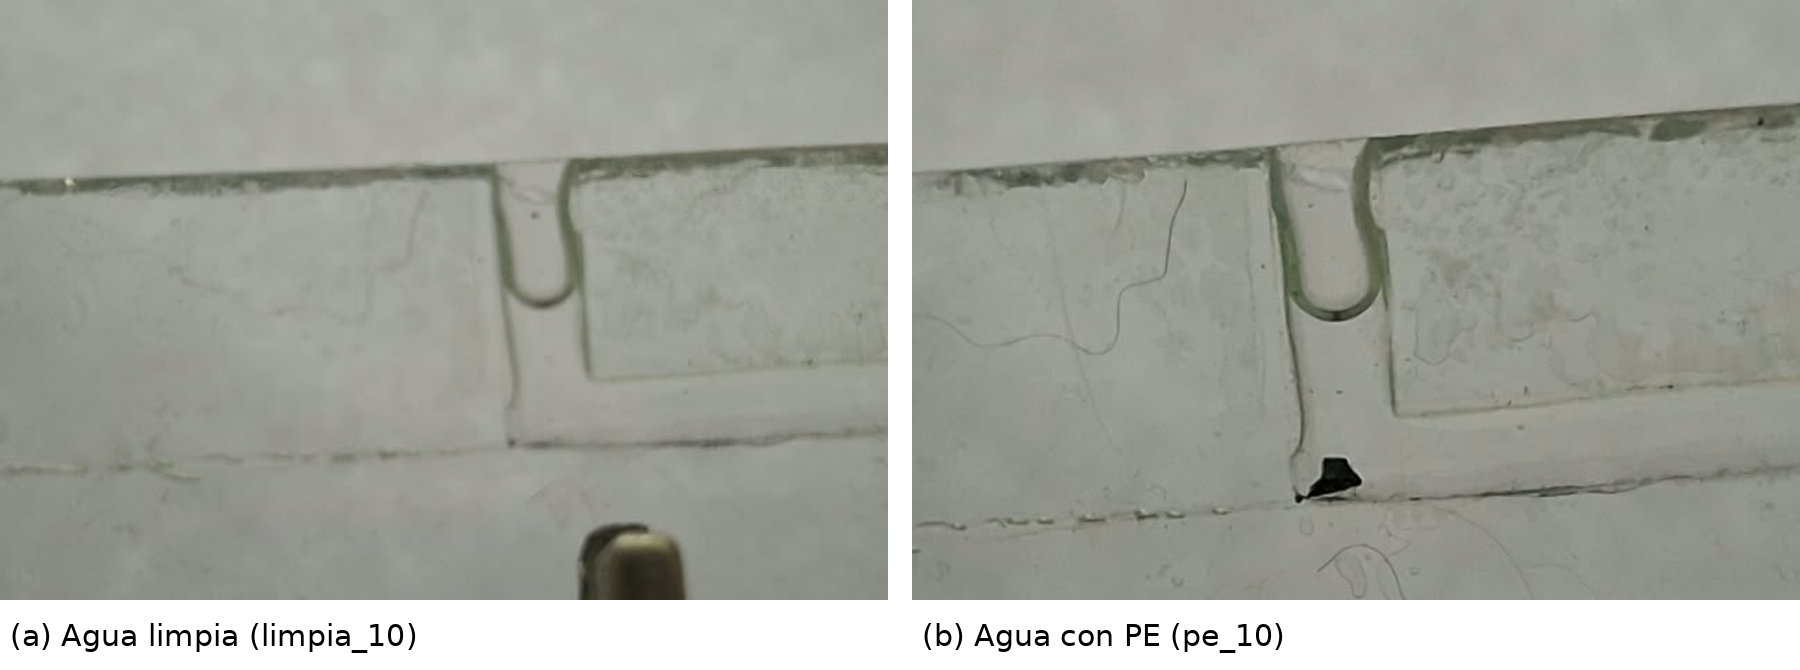
\includegraphics[width=\textwidth]{figuras/fotos_zona_medicion.png}
  \caption{Fotografías a contraluz de la zona de medición del chip~2: (a) llenado con
    agua limpia, $T_{\mathrm{rel}} = 93{,}7\,\%$; (b) llenado con partículas de PE, en el
    que se observa una partícula en la esquina del canal, $T_{\mathrm{rel}} = 20{,}5\,\%$.}
  \label{fig:fotos_zona}
\end{figure}
